% Imported from topics/video-generation/seedance-2.5/editing-conditions.md
\chapter{源条件与统一编辑接口}\label{seedance-m17}
\moduleinfo{M17}{候选设计与工程选型；组合效果待验证}{\hyperref[src-vace]{\texttt{vace}}、\hyperref[src-videocof]{\texttt{videocof}}、\hyperref[src-vincie-next]{\texttt{vincie-next}}、\hyperref[src-ltx-2]{\texttt{ltx-2}}}

编辑的变化范围已经明确，这里把源内容、区域与目标分别写成主干可以接收的条件。

编辑再细看，会遇到连续三个未知量：指令中的对象是谁，哪一片区域需要变，这种变化怎样沿时间传播？若只送入源视频和一句指令，三者都藏在同一个隐含过程里，失败后难判断哪一步出了问题，数据也难以分别监督。

所以这里把用户给定条件、预测区域与生成目标分开，仍由共同视频主干处理。先写出这些对象的关系，再决定各自从哪条支路进入网络。

\section{用帧与 mask 表示不同任务}\label{seedance-m17-ux7528ux5e27ux4e0e-mask-ux8868ux793aux4e0dux540cux4efbux52a1}

设源条件为 \(F\)，编辑 mask 为 \(M\)，其中 \(M=1\) 表示允许重新生成。可将条件分成两路：

\[
F_c=F\odot M,\qquad F_k=F\odot(1-M).
\]

\(F_c\) 放待改变内容或控制信号，\(F_k\) 放必须保留的信息。分别编码后，再连同压缩到相同网格的 mask 进入条件支路：

\[
C_{\mathrm{edit}}=P\bigl[E_v(F_c);E_v(F_k);D(M)\bigr].
\]

源内容先拆成待变与保留两路，再各自编码，最后与对齐的 mask 拼接并投影。目标 noisy latent 另走原输入，因此条件表示和生成目标在这一步并没有混成同一个张量。这个区分也解释了为什么新增支路可以不改旧输入头。

分号表示通道拼接，\(D\) 表示保持对齐的 mask 变换。目标的带噪 latent 仍走原主干输入，新增条件支路在选定层提供残差信息，不直接改写旧 checkpoint 的输入通道。

\begin{figure}
\centering
\pandocbounded{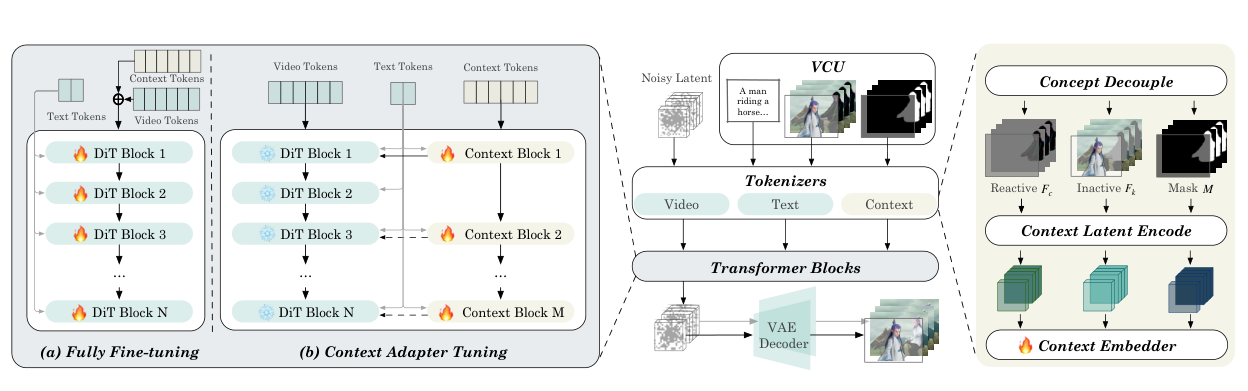
\includegraphics[keepaspectratio,alt={视觉条件的拆分、编码与主干残差连接 （论文示意，来源：vace）}]{assets/seedance/figures/unified-context.png}}
\caption{视觉条件的拆分、编码与主干残差连接 （论文示意，来源：vace）}
\end{figure}

这套表示可以覆盖几种任务：空条件和全生成 mask 对应文生视频；源帧与全生成 mask 对应重绘；源帧与局部 mask 对应局部编辑；历史帧可作为续写条件。它们使用相近接口，却仍需要各自的训练样本，表示统一不能推出任务能力自然齐全。

\section{时间和空间需要同时定义}\label{seedance-m17-ux65f6ux95f4ux548cux7a7aux95f4ux9700ux8981ux540cux65f6ux5b9aux4e49}

用户要求``第二到第四秒更换角色 A 的外套''时，最终编辑范围可写为：

\[
M(\tau,y,x)=M_{\mathrm{coat},A}(\tau,y,x)
\cdot\mathbf{1}_{[2,4)}(\tau).
\]

模型要读取边界上下文，因此工作区按 VAE 和 patch 感受野适当扩张；最终交付的替换范围仍由用户要求决定。若还要让阴影、光照或遮挡一起变化，就继续说明这些影响是否被允许，不能只靠一个对象框代表所有约束。

源视频、参考图、区域条件与目标各自编码，避免不连续素材在因果 VAE 中互相影响。loss mask、条件 mask 与最终 alpha 也分开保存，它们虽然来自同一个任务范围，承担的计算含义却不同。

\section{用户不提供 mask 时，先定位再编辑}\label{seedance-m17-ux7528ux6237ux4e0dux63d0ux4f9b-mask-ux65f6ux5148ux5b9aux4f4dux518dux7f16ux8f91}

例如指令只说“删除右边穿绿衣的人”，没有给 mask。此时先找区域，再生成结果，关系更清楚。区域可表示成分割 mask，也可用突出该区域的灰度帧，关键是它应当能被检查和监督。

\begin{figure}
\centering
\pandocbounded{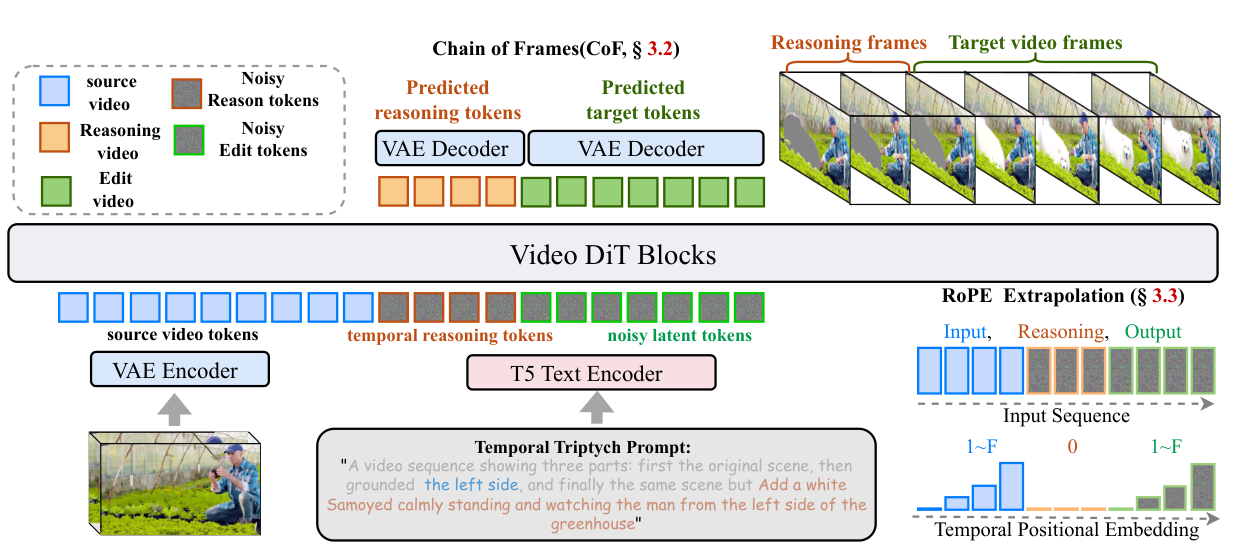
\includegraphics[keepaspectratio,alt={源内容、区域表示和目标内容的链式组织 （论文示意，来源：videocof）}]{assets/seedance/figures/reason-edit.png}}
\caption{源内容、区域表示和目标内容的链式组织 （论文示意，来源：videocof）}
\end{figure}

这里说的区域“推理”有一个可见的中间结果，不等于语言模型内部的隐藏思维。首版先把它写成两个阶段：

\begin{verbatim}
源视频 + 指令 → 目标区域/关键帧示意
源视频 + 已确认区域 + 指令 + 参考 → 编辑后视频
\end{verbatim}

若用户已经给了可靠 mask，可直接做第二阶段；自动定位置信度低时，再让用户修正。训练生成阶段也逐渐加入预测区域，才能面对定位误差。若永远只读完美真值，推理时一点越界就可能改变生成条件。

VideoCoF 则把区域与目标放进联合去噪序列，源 latent 保持干净，区域和目标共同监督。本文先采用显式两阶段，便于检查和返工，但多付一次定位或生成开销。这是两种执行图，不能只因为都预测区域就说它们相同。

\section{编辑示例图怎样减少成对视频数据需求}\label{seedance-m17-ux7f16ux8f91ux793aux4f8bux56feux600eux6837ux51cfux5c11ux6210ux5bf9ux89c6ux9891ux6570ux636eux9700ux6c42}

还可以先从源视频选关键帧 \(I_s\)，将它编辑为 \(I_t\)，再让整段视频读取``修改前、修改后''的图像示例：

\[
p(V_t\mid V_s,c,I_s,I_t).
\]

编辑前后图像给出了一个具体变换，因而可以利用较多图像编辑数据。接到视频后，目标还要保持源运动；若只按修改后图片重新生成另一段动作，就没有完成从示例传播编辑的任务。

关键帧能说明正面外观，不一定说明转身后的背面，也未必覆盖后半段才出现的道具或多角色关系。这些情况仍需增加参考或编辑示例。若各角度独立编辑后直接拼接，单帧都合理，时间上也可能互相冲突。

\section{损失怎样分配}\label{seedance-m17-ux635fux5931ux600eux6837ux5206ux914d}

源视频是条件，不作为普通噪声目标。目标视频使用有效位置上的流匹配损失；若训练区域预测，再给区域头或区域 latent 单独监督：

\[
\mathcal{L}=\mathcal{L}^{\mathrm{target}}_{\mathrm{flow}}
+\lambda_r\mathcal{L}_{\mathrm{region}}
+\lambda_p\mathcal{L}_{\mathrm{preserve}}.
\]

保持项的前提是空间仍可对齐。改相机、视角或大姿态时，逐像素拉回原图可能正好阻止目标变化。区域预测和生成质量因此要分别看，保持误差小也可能只是模型选择了不编辑。

\section{最终输出怎样保护已通过的部分}\label{seedance-m17-ux6700ux7ec8ux8f93ux51faux600eux6837ux4fddux62a4ux5df2ux901aux8fc7ux7684ux90e8ux5206}

严格局部任务最后可只合成允许区域，外部取原像素；需保留的音轨直接取原采样。这样保持由输出合成实现，不再要求有损 VAE 在未编辑处做到无损重建。

语义编辑则允许更多上下文变化，应按身份、动作、几何与连贯性验收。先做``颜色/局部替换''，再做视角和光照任务，能更清楚地定位接口是否有效。

机制代码见 \hyperref[code-condition-unit]{condition\_unit.py} 与 \hyperref[code-local-edit]{local\_edit.py}，均只作说明。真实统一条件实现读 \href{https://github.com/ali-vilab/VACE}{VACE}，区域中间表示读 \href{https://github.com/knightyxp/VideoCoF}{VideoCoF}，图像编辑迁移到视频的方法读 \href{https://vincie-next.github.io/}{VINCIE-NExT}。它们提供可借鉴机制，迁入联合音视频主干仍需要新适配和训练。
